
\documentclass[12pt, letterpaper]{article}

\usepackage{enumitem}
\setlist{  
  listparindent=\parindent
}
\usepackage{graphicx}
\graphicspath{ {./Images/}}
\usepackage{dsfont}
\usepackage{array}
\usepackage{witharrows}
\usepackage{amsmath}
\usepackage{amssymb}
\usepackage{amsthm}
\usepackage{mathtools}
\usepackage[utf8]{inputenc}
\usepackage{geometry}
\usepackage{tikz, pgfplots}
\usetikzlibrary{positioning, arrows.meta}
\usepackage{tabularx}
\usepackage{siunitx}
\usepackage{fullpage}
\usepgfplotslibrary{fillbetween} 


\newtheorem{theorem}{Theorem}[section]
\newtheorem{proposition}{Proposition}[section]
\newtheorem{corollary}{Corollary}[theorem]
\newtheorem{lemma}[theorem]{Lemma}

\theoremstyle{definition}
\newtheorem{definition}{Definition}[section]

\theoremstyle{remark}
\newtheorem*{remark}{Remark}

\theoremstyle{definition}
\newtheorem*{example}{Example}

\newlength{\conditionwd}
\newenvironment{conditions*}
  {\par\vspace{\abovedisplayskip}\noindent
   \tabularx{\columnwidth}{>{$}l<{$} @{\ : } >{\raggedright\arraybackslash}X}}
  {\endtabularx\vspace{\belowdisplayskip}}

\newcommand{\norm}[1]{\left\lVert #1 \right\rVert}
\newcommand{\bb}[1]{\mathbb{#1}}
\newcommand{\pd}[2]{\frac{\partial #1}{\partial #2}}

\title{BLP Midterm Report}
\author{Stephen Min}
\date{}

\begin{document}
\maketitle

\section{BLP Estimation}
\subsection{Data Merging}
All the modified data was prepared using R. The markdown file should contain adequate documentation of what happened to the data. In short, all the necessary data was converted into long format and merged to be compatible with the original BLP code.

A screenshot of part of the merged demand data will be on the last page.

\subsection{Estimation with Provided Instruments}
Below is a table of the estimated parameters, rounded to 3 decimal places so that the table isn't too ugly:

\begin{table}[ht]
    \centering
    \begin{tabular}{|c|c|}
        \hline
        \textbf{Parameter} & \textbf{Estimate} \\ \hline
        $\theta_1$  & $[-1.611, 2.045]$ \\ \hline
        $\theta_2$  & $[0.155, 0.589]$ \\ \hline
        $\theta_3$  & $[0.006]$ \\ \hline
    \end{tabular}
\end{table}

The first entry of $\theta_1$ is for price, while the second is for caffeine score. The entries of $\theta_1$ are a bit hard to interpret on their own, but the $\exp()$ of the coefficients can be roughly thought of as, for a given consumer, the number that relative probability of choosing a given good over the base alternative is multiplied by for a one unit increase in the respective covariate. 

For example, if the price of good $j$ increases by $\$1$, then we should expect that the relative probability of a given individual choosing good $j$ over the baseline alternative (usually defined as not buying anything) to be multiplied by $\exp(-1.611)$ in this case. 

$\theta_3$ has an easier interpretation. Since MC was assumed to take the form of
\[
	\ln(MC_{j})=w_{j}\theta_{3}+\omega_{j},
\]
we can think of $\theta_3$ as a roughly $0.6\% $ increase of MC for a one unit change in $w$.

\newpage

\subsection{Estimation with Generated Instruments}

\begin{table}[ht]
    \centering
    \begin{tabular}{|c|c|}
        \hline
        \textbf{Parameter} & \textbf{Estimate} \\ \hline
        $\theta_1$  & $[ -1.606, 2.032]$ \\ \hline
        $\theta_2$  & $[0.258, 0.589]$ \\ \hline
        $\theta_3$  & $[0.006]$ \\ \hline
    \end{tabular}
\end{table}

Estimation with the generated instruments provided almost the same parameters. $\theta_3$ did not have any generated instruments, so it was estimated with OLS. Only $\theta_2$ had a noticeably different estimate for the variation associated with price. I'm honestly not sure why. It may be something to do with the weighting matrix changing.

\section{Merger Simulation}

The data for a hypothetical McHorton's was prepared with the same R file. The code to simulate new prices is in the Supply.jl file. 

I used the fixed-point solver from NLsolve to estimate the counterfactual prices. I first tried the chosen method on the original prices to see if it would give the same prices back. In general, there's no guarantee that a fixed point algorithm would converge to p, but in this situation it appears to have worked well.

Assuming that my results are somewhat accurate, the merger simulation showed that over 400 prices would be lower for both scenarios, meaning that as a regulator I'd probably approve of the merger.

\section{Some Notes}
\begin{itemize}
	\item Julia 1.6.4 (and some other versions around there) has some kind of bug with solving equations involving large matrices. I had to update Julia to get my fixed point function to work (it would give a StackOverFlowError with no details).
	\item The OLS and Derivative files weren't touched, but they're still in the code folder.
	\item Aside from what's mentioned in the main sections, all the code was modified according to the new dimensions of the data.	
\end{itemize}


\begin{center}
	\begin{figure}
		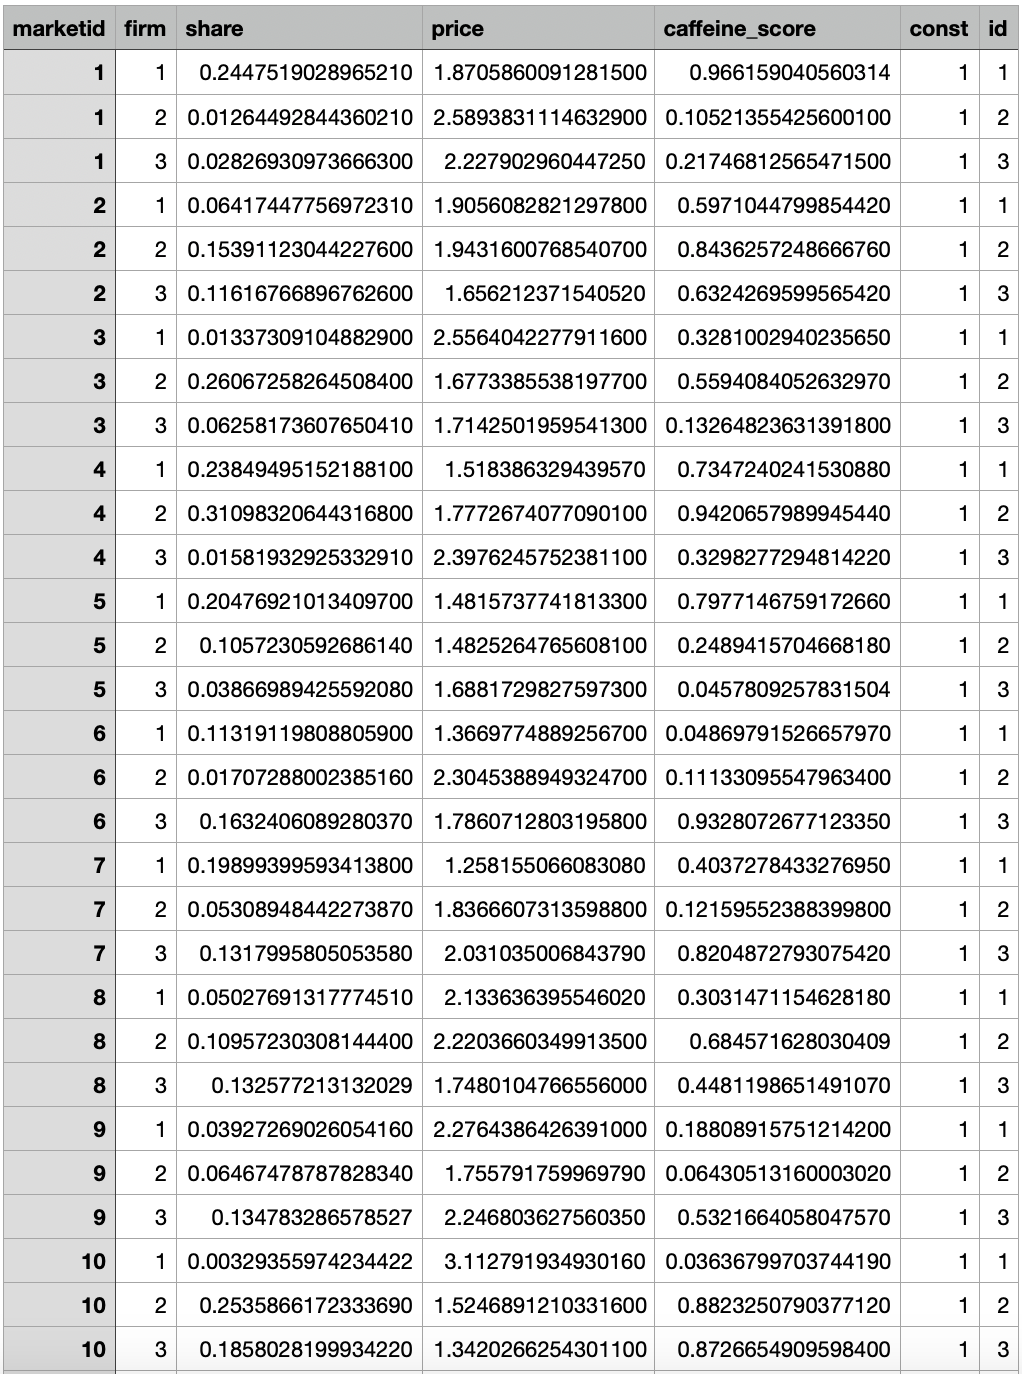
\includegraphics{mergeddata.png}
	\end{figure}
\end{center}

\end{document}